\subsection{Teil V. Erzielung einer nahezu optimalen Regelungsleistung}
\label{subsec:Achievement_of_Near-Optimal_Control_Performance}

Während der entscheidenden Endphase des Trainingsprozesses verzeichneten wir bei einem unserer Modelle, welches wir im Folgenden als Modell X bezeichnen, eine stetige Verbesserung der Regelungsleistung. Diese Beobachtung wird durch die in Abbildung \ref{fig:phase 2 whole lern process} dokumentierte, kontinuierliche Leistungssteigerung bestätigt. Durch konsequente Feinabstimmung und die Auswahl der leistungsfähigsten Modelle zu verschiedenen Zeitpunkten des Trainings konnte ein herausragendes Ergebnis erzielt werden: Das Modell X erreichte eine maximale Belohnung von -3.99. Dies deutet auf eine Performance hin, die dem optimalen Steuerungsverhalten sehr nahekommt.

\begin{table}[htbp]
\centering
\caption{Maximale Leistung des Modells X nach umfangreichen Trainingsiterationen}
\label{tab:maximum_performance_model_x}
\begin{tabular}{l c}
\hline
\textbf{Parameter} & \textbf{Wert} \\
\hline
Iteration & Geschätzt \\
Belohnung & -3.9928830028461824 \\
Aktion & [434.82286483, 91.83493555, 1.52657181] \\
Induktivität & \( 5.0 \times 10^{-3} \) \\
Kapazität & \( 10.0 \times 10^{-6} \) \\
\hline
\end{tabular}
\end{table}

\begin{figure}[htbp]
\centering
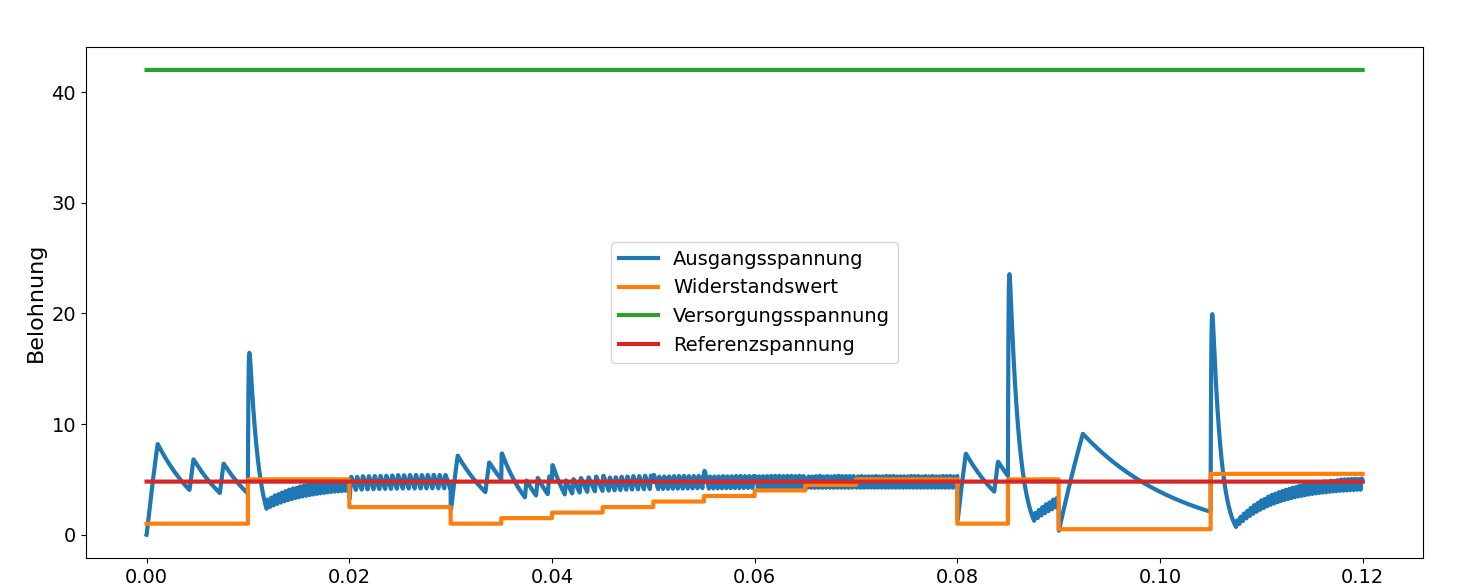
\includegraphics[width=\textwidth]{4Ergebnisse/Phasen/2Phase/TeilV.png}
\caption{Darstellung der finalen Leistungssteigerung des Modells X, welche die nahezu optimale Regelungsleistung illustriert.}
\label{fig:final_performance_model_x}
\end{figure}

Die Erreichung einer solch hohen Belohnung nach einer langen Reihe von Trainingsiterationen bestätigt die Effektivität unseres Ansatzes zur Modelloptimierung. Die Performance \ref{fig:final_performance_model_x} von Modell X stellt einen bedeutenden Meilenstein dar, der zeigt, dass das Modell nicht nur theoretisch, sondern auch in der simulierten Anwendung in der Lage ist, sich effektiv anzupassen und zu optimieren. Dieses Ergebnis betont die Relevanz und Präzision unserer Belohnungsfunktion sowie die Robustheit des DDPG-Modells unter komplexen und anspruchsvollen Bedingungen.

